\documentclass[12pt,a4paper]{report}
\usepackage[utf8]{inputenc}
\usepackage{amsmath}
\usepackage{amsfonts}
\usepackage{amssymb}
\usepackage{graphicx}
\usepackage{float}
\input defs.tex
\bibliographystyle{alpha}
\graphicspath{ {./figures/} }
\hyphenpenalty=10000

\title{Game Theoretic Solutions to Multiple Antenna Power Control in Heterogeneous Networks}
\author{Peter Hartig}

\begin{document}
\maketitle
\begin{abstract}
This work investigates resource allocation strategies for a communication system with uncoordinated users and MIMO capable base stations. Following a game theoretic , it is shown that unlike SISO case investigated in \cite{ghosh2015normalized}, the general MIMO problem does not admit the N-Concave game framework. Refinements of the general problem are then made to use the N-Concave game framework. These refinements require pre-selection of transmission beam-formers prior to the allocation of power and therefore the beam-former design is also considered to increase the achievable player utility. These results are verified and further analyzed in simulations.
\end{abstract}
%
%\newpage
\tableofcontents


\chapter{Introduction}
Modern communication systems often incorporate numerous, uncoordinated users competing for a limited resource. In this work, a game theoretic approach considers a wireless communication network with uncoordinated macrocell users and femtocell base stations. The goal of this approach is to find Nash Equilibrium in which femtocell base stations optimize individual utility while ensuring interference tolerances are not violated for macrocell users. 
Previous work has shown solutions for systems in which femtocell base stations transmit over a single input, single output (SISO) channel; therefore the multiple input, multiple ouput (MIMO) case is investigated here. 
\par
This work focuses on achieving Nash Equilibrium (NE) using distributed solutions. In the communications context, distribution of system optimization is preferable in order to minimize the amount of information passing overhead often required by central optimization. 


\section{Notation}
The following notation is used throughout the remainder. 
$E[x]$ is the expected value of a random variable $x$.
Vectors are denoted by bold font, lower-case letters ($\mathbf{x}$) and are assumed to be column vectors.
Matrices are denoted by bold font, upper-case letters ($\mathbf{X}$). The transpose and hermetian of $\mathbf{X}$ are denoted by $\mathbf{X}^T$ and $\mathbf{X}^H$ respectively.
$\mathbf{I}$ denotes the identity matrix.


\section{Relevant Tools/Theory}\label{tools}
It is useful to first review relevant game theoretic tools. Together, these tools provide a series of steps to follow in solving for Nash Equilibrium via distributed solutions. 

\begin{enumerate}
\item The Concave N-Person game: A framework for proving existence and uniqueness of NE.

\begin{itemize}
\item
\textbf{Definition:} A game in which individual players maximize a concave utility function over a convex strategy set resulting from problem constraints (potentially player coupled). 
\item 
\textbf{Existence of Nash Equilibrium:} Pure Strategy NE exist for Concave N-Person  games \cite[Thm1]{rosen1964existence}. 
\item
\textbf{Uniqueness of Nash Equilibrium:} To prove uniqueness of NE for Concave N-Person  games, the Normalized Nash Equilibrium is introduced.
First, take a weighted sum of the player utility functions $U_{\mathrm{f}}(b_{\text{f}})$.
\begin{equation*}
\sigma(\mathbf{b},\mathbf{r})  = \Sigma_{\mathrm{f=1}}^{\mathrm{F}} r_{\mathrm{f}}U_{\mathrm{f}}(b_{\text{f}}),\; \mathbf{r}=(r_{\text{1}}... r_{\text{F}})
,\; \mathbf{u}=(b_{\text{1}}... b_{\text{F}})
, \; 
r_{\mathrm{f}} \geq 0.
\end{equation*}
The gradient of $
\sigma(\mathbf{b},\mathbf{r})$
is  
\begin{equation}
g(b,r)= 
\begin{bmatrix}
r_1 \nabla U_{1}(b_1)
\\
r_2 \nabla U_{2}(b_2)
\\
\vdots\\
r_F \nabla U_{\text{F}}(b_{\text{F}})
\end{bmatrix}.
\end{equation}
 The matrix valued function $G(b,r) $ is defined as the Jacobian of $g(b,r) $.



Negative Definiteness of the matrix $[G(b,r)+G^{T}(b,r)] $ is a sufficient condition for Diagonally Strict Concavity of $\sigma(\mathbf{b},\mathbf{r})$ which is a sufficient condition for uniqueness of a NNE \cite[Thm4]{rosen1964existence}.


\end{itemize}
\item The Potential Function: An equivalent but central optimization problem representing a game.
\begin{itemize}
\item
\textbf{Definition:}  A function
$ \Psi(b_{\text{f}})$ which satisfies:
\begin{equation}\label{potential_game_condition}
\frac{\partial \Psi(\mathbf{b})}{\partial b_{\text{f}}}
 =
 \frac{\partial U_f(b_{\text{f}})}{\partial b_{\text{f}}},
 \;\textbf{b}=[b_{1}, b_2... b_{\text{F}}]
\end{equation} 
for a game with player utility functions $U_f(b_{\text{f}})$.
In words, $ \Psi(\mathbf{b})$ is a function whose gradient with respect to the strategy $b_{\text{f}}$ of a player, is equal to the gradient of that player's utility function with respect to $b_{\text{f}}$.
\item \textbf{Result 1:} Global optima of a potential function are Nash Equilibrium \cite{monderer1996potential}.
\item \textbf{Result 2:} For a Concave N-Person games admitting a potential function, the potential function is concave; allowing for use of convex optimization tools to find a NE. 
\end{itemize}



\item Distributed Optimization: Solving a central optimization problem using multiple processes in parallel.
In particular, the Dual Ascent method described in \cite{boyd2011distributed} is used in this work.

\textbf{Distributed Dual Ascent:} 
\begin{itemize}
\item For a central optimization problem (obtained using a Potential Function in this work), determine the dual problem to the central, primal problem.
\item Evaluate if the dual problem can be separated into sub-problems; each with independent optimization variables.
\item Perform an ascent of the dual problem by iterating the following:
\begin{enumerate}
\item Solve the separate dual function of the sub-problems.
\item Broadcast these solutions and perform the gradient step of the dual problem.
\end{enumerate}
\end{itemize}

If the problem is convex with strong duality, the dual ascent will converge to the optimal (in this case a Nash Equilibrium).

\end{enumerate}




\section{Outline}
The above tools are used in the steps outlined below. 
\begin{itemize}
\item 
\ref{genmodel}: Introduce the system model for the general game.
\item 
\ref{genproblem}: Analyze the general setup to see why further refinements are useful in arriving at a distributed solution. 
\item
\ref{conmodel}: Introduce refinements to the system model.
\item 
\ref{conproblem}: Develop a distributed solution using the refined system model.
\item 
\ref{numerical}: Discuss numerical results of the proposed solution. 
\end{itemize}
\chapter{System Model}

\section{General System Model}\label{genmodel}

\subsection{Players: Femtocell Base Stations}


Each player of the game, a femtocell base station (FBS) $\text{f} \in \{1 ... F\}$ , is characterized by the following.
\begin{itemize}
\item 
$T_{\text{f}}$ antennas with which to transmit to $K_{\text{f}}$ femtocell users (it is assumed that $T_{\text{f}} \geq K_{\text{f}}$).
\\
\item 
	The beamforming matrix $\mathbf{U}_{\mathrm{f}} \in \mathbb{C}_{T_{\text{f}} \times K_{\text{f}}}$ such that the transmitted 		
	signal is $\mathbf{s}_{\mathrm{f}
	}= \mathbf{U_{\mathrm{f}}}\mathbf{x_{\mathrm{f}}}$. The 		
	vector of symbols for users of FBS $\text{f}$, $\mathbf{x_{\mathrm{f}}}$, is  normalized such that $E[\|x_{\mathrm{f,i}}
	\|_2^2]=1$ and $E[\mathbf{x}_{\mathrm{f}}\mathbf{x}_{\mathrm{f}}^H]=\mathbf{I}_{K_{\text{f}} \times K_{\text{f}}}$.
\\
\item 
	The power constraint $trace(\mathbf{U}_{\text{f}}^H\mathbf{U}_{\text{f}}) \leq P^{Total}_{\text{f}} $.

\item 
	The cost function $U_{\text{f}}() =
	\sum_{\mathrm{i=1}}^{\mathrm{K_{\text{f}}}}
    	 U_{\mathrm{f,i}}(\gamma_{\mathrm{f,i}}) $
    	in which all $U_{\mathrm{f,i}}()$ are non-decreasing (no convexity assumption is made at this point).

\item 
	Perfect knowledge of the downlink channel matrix $\mathbf{H_\mathrm{f}} \in \mathbb{C}_{K_{\text{f}} \times T_{\text{f}}} $ to the $K_{\text{f}}$ FBS users.
% TODO(Simulate degradation with incomplete CSI solution?)
\\
\item
	 FBSs are assumed to be spaced far apart in distance such that FBS $\text{f}$ 
	 causes no interference to the users of any other FBS.
\end{itemize}

\subsection{Macrocell Users}
Macrocell users $m \in \{1 ... M\}$ introduce constraints into the game. These users are characterized by the following.

\begin{itemize}
\item 
	Received interference constraint
	$\sum^F_{\text{f}=1} \mathbf{\tilde{h}}_{\mathrm{m,f}}^T  \mathbf{U_{\mathrm{f}}} 						
	\mathbf{U_{\mathrm{f}}^{\mathrm{H}}} \mathbf{\tilde{h}_{\mathrm{m,f}}^*} \leq I^{Threshold}		
	_{\mathrm{m}} $. In which $\mathbf{\tilde{h}}_{\mathrm{m,f}}$ is the channel from FBS $\text{f}$ to macro user $\text{m}$

\item 
	FBS $\text{f}$ is assumed to know the downlink channel matrix $\tilde{\mathbf{H}_{\mathrm{f}}} \in \mathbb{C}_{M \times T_{\text{f}}}$ to all $M$ Macrocell users.
\\
\end{itemize}

\subsection{Femtocell Users}
\begin{itemize}

\item User $i$ of FBS $f$ has signal to interference plus noise ratio (SINR):
	\begin{equation*}
	\gamma_{\mathrm{f,i}} = \frac{\|\mathbf{h^H_{\mathrm{f,i}}u_{\mathrm{f,i}}}\|^2}
	{\sigma^2_{\text{noise}}   +
	\underbrace{
	 \sum_{\mathrm{\tilde{f}}=1,\mathrm{\tilde{f}}\neq f}^{\mathrm{F}} \sum_{\mathrm{u=1}}^{K_{\mathrm{\tilde{f}}}}
	\|\mathbf{h^H_{\mathrm{\tilde{f},u}}u_{\mathrm{\tilde{f},i}}}\|^2}_{\mathrm{inter-cell}}
	 + 
	 \underbrace{
	 \sum_{\mathrm{\tilde{k}\neq i}}^{\mathrm{K_f}}
	 \|\mathbf{h^H_{\mathrm{f,\tilde{k}}}u_{\mathrm{f,\tilde{k}}}}\|^2}_{\mathrm{intra-cell}}},
	  \; \mathrm{i \in \{1 ... K_f\}}
	  \end{equation*}
\\
with noise power $\sigma^2_{\text{noise}}.$
\\

By the FBS spacing assumption above, this reduces to:
	\begin{equation*}
	\gamma_{\mathrm{f,i}} = \frac{\|\mathbf{h^H_{\mathrm{f,i}}u_{\mathrm{f,i}}}\|^2}
	{\sigma^2_{\text{noise}} 
	 + \sum_{\mathrm{\tilde{k}\neq i}}^{\mathrm{K_f}}
	  \|\mathbf{h^H_{\mathrm{f,\tilde{k}}}u_{\mathrm{f,\tilde{k}}}}\|^2},
	  \; \mathrm{i \in \{1 ... K_f\}}
	\end{equation*}
\\


\end{itemize}





\subsection{General Optimization Problem}\label{genproblem}

Each FBS $\text{f}$ attempts to maximize utility function $U_{\text{f}}()$ while satisfying the interference constraints imposed by the macrocell users and a transmission power constraint. The results in the following optimization problem at each FBS.
\par

	\begin{subequations}
	\label{optim}
	\begin{align}
	    \underset{\mathbf{U}_{\mathrm{f}} }{\text{minimize: }} \;
	    & - \sum_{\mathrm{i=1}}^{\mathrm{K_f}}
    	U_{\mathrm{f,i}}(\gamma_{\mathrm{f,i}}) \label{player_opt} \\
	    \text{subject to: } \; &
	   \sum^F_{f=1} \mathbf{\tilde{h}}_{\mathrm{m,f}}^T  \mathbf{U_{\mathrm{f}}}		
	\mathbf{U_{\mathrm{f}}^{\mathrm{H}}} \mathbf{\tilde{h}_{\mathrm{m,f}}^*} \leq I^{Threshold}		
	_{\mathrm{m}} & m \in \{1 ...M\} 
		\label{interference_const_gen}\\
        & trace(\mathbf{U}_{\text{f}}^H\mathbf{U}_{\text{f}}) \leq P^{Total}_{\text{f}} \label{power_const_gen}\\
        & \langle \mathbf{h_{\text{f,j}}}\mathbf{u_{\text{f,i}}} \rangle =0\ & \; \forall \; \text{j} \in \{1... K_{\text{f}}\}\backslash \text{i} ,\; \forall \; \text{i} \in \{1 ... K_{\text{f}}\} \label{zf_const_gen}
	\end{align}
	\end{subequations}


Constraint \eqref{zf_const_gen} restricts $\mathbf{U}_{\mathrm{f}}$ such that  
	\begin{equation}\label{zf_snr}
	\gamma_{\mathrm{f,i}} = \frac{\|\mathbf{h^H_{\mathrm{f,i}}u_{\mathrm{f,i}}}\|^2}
	{\sigma^2_{noise}  
	}
	= 
	\frac{\mathbf{u^H_{\mathrm{f,i}}h_{\mathrm{f,i}}h^H_{\mathrm{f,i}}u_{\mathrm{f,i}}}}
	{\sigma^2_{noise}  
	}.
	\end{equation}
	As a result, $U_{\mathrm{f,i}}(\gamma_{\mathrm{f,i}}) $ is concave with respect to $\gamma_{\mathrm{f,i}}$.
	
\subsection{Concave N-Person game analysis of general setup}
The convexity of the resulting problem is analyzed to investigate if this system admits the Concave N-Person game framework described above. 

\begin{enumerate}


\item
First, check that the constraints form a convex, closed and bounded set. 

\begin{itemize}

\item
	Constaint \eqref{interference_const_gen} contains $M$ quadratic constraints on $\mathbf{U_f}$, each of which 
	can be rewritten  as

\begin{gather*}
	\sum_{f=1}^F
	trace(\mathbf{U_f^H} \mathbf{\tilde{h}_{m,f}} \mathbf{\tilde{h}_{m,f}^H} \mathbf{U_f} )\leq 
	I^{Threshold}_{m}.
\end{gather*}
This can be further decomposed into  
	\begin{gather*}
	\sum_{f=1}^F
	\sum_{i=1}^{f_i}
	\mathbf{u_{\mathrm{f,i}}^H}\mathbf{\tilde{h}_{\mathrm{m,f}}} \mathbf{\tilde{h}}_{\mathrm{m,f}}^H
	\mathbf{u_{\mathrm{f,i}}} \leq I^{Threshold}_{m}
	\end{gather*}
in which the matrix $ \mathbf{\tilde{h}_{\mathrm{m,f}}} \mathbf{\tilde{h}}_{\mathrm{m,f}}^H$ is  positive semi-definite creating in a convex set 
\cite[p.~8,9]{BoV:04}. 
%This is essentially high dimensional ellipsoid.


\item \
	Constraint \eqref{power_const_gen} can be similarly decomposed into the sum
	\begin{gather*}
		\sum_{i=1}^{K_f}\mathbf{u_{\mathrm{f,i}}^{\mathrm{H}}} \mathbf{I} 		
		\mathbf{u_{\mathrm{f,i}}} \leq  P^{Total}_{f}
	\end{gather*}
	in which $\mathbf{I}$ is positive definite, creating a strictly convex set.

\item 
	Constaint \eqref{zf_const_gen} is an affine constraint. 
		\begin{gather*}
		\langle \mathbf{h_{\mathrm{f,j}}}\mathbf{u_{\mathrm{f,i}}} \rangle =0
		\end{gather*}
%Note that affine constaints to not have to satisfy Slater's condition
\end{itemize}


\item Second, check if the utility function is concave.
\begin{itemize}
\item 
With
	\begin{equation*}\label{zf_snr}
	\gamma_{\mathrm{f,i}} = 
	\frac{\mathbf{u^H_{\mathrm{f,i}}h_{\mathrm{f,i}}h^H_{\mathrm{f,i}}u_{\mathrm{f,i}}}}
	{\sigma^2_{noise}  
	},
	\end{equation*}
	 $\mathbf{h}_{\mathrm{f,i}}\mathbf{h}^H_{\mathrm{f,i}}$ is positive semi-definite so $\gamma_{\mathrm{f,i}}$ is convex in ${\mathbf{u}_{\mathrm{f,i}}}$. 
	 The resulting composition $U_{\mathrm{f,i}}(\gamma_{\mathrm{f,i}}) $ is concave only if $U_{\mathrm{f,i}}() $ is concave and non-increasing; violating the non-decreasing definition of $U_{\mathrm{f,i}}() $.
If $U_{\mathrm{f,i}}() $ is a general, non-decreasing function, the result is quasiconvex \cite[p.~102]{BoV:04}. If $U_{\mathrm{f,i}}() $ is  non-decreasing and convex, the resulting
   function is convex and therefore, Concave Programming can be used to find a \emph{maximum}.
\end{itemize}

\end{enumerate}

\subsection{Potential Game for General Problem}
Under the current system model, the game is not a Concave N-Person game. Nevertheless, because of the independence of the utility functions due to the spacing assumption, the game still admits a potential function. Investigation of potential distributed, Concave Programming techniques for solving this problem is left for future work. 

\section{Concave System Model}\label{conmodel}

The general setup of this game seen in the previous section prohibits the use of established tools to reach a NE.
The following refinement of the system model permits a unique NE to be found via a single convex problem which may be distributed across across base stations and users in the network.
\par
Rather than jointly optimizing the power allocation over the set of all zero-forcing beamformers, we now pre-select normalized, zero-forcing beamformers independently, \emph{before} the allocation of power.
As seen later, one result of this ordering is that additional degrees of freedom at the FBS cannot be exploited with knowledge of the final power allocation. 

\subsection{Players: Femtocell Base Stations}
Femtocell Base Stations are adapted from the general setup to the refined setup by the following.
\begin{itemize}
\item 
	FBSs with multiple antennas ($T_f \geq 1$) can beamform their transmission using the precoding 	
	matrix $\mathbf{U}_{\mathrm{\text{f}}} \in \mathbb{C}_{T_{\text{f}} \times K_{\text{f}}}$ .
	The columns of $\mathbf{U}_{\mathrm{f}}$ are now \emph{normalized} such that 
	 $\|\mathbf{u}_{\mathrm{fi}}\|^2 =1 \;\forall i \in \{1 ... K_{\text{f}}\}$.
\\

\item 
$\mathbf{U}_f$ is selected as a pseudo-inverse to $\mathbf{H_\mathrm{f}}$.
Such that
\begin{gather*}
\mathbf{H}_{\mathrm{f}}  \mathbf{U_{\mathrm{f}}} = \mathbf{I}.
\end{gather*} 


\item  
	FBS $\text{f}$ allocates transmission power using the diagonal, power allocation  	
	matrix $\mathrm{diag}(\mathbf{p}_{\mathrm{f}})$ with $p_{\mathrm{fi}} \geq 0, \forall i \in \{1 ... K_{\text{f}}\}$
such that the transmitted 		
	signal is 
	$\mathbf{s}_{\mathrm{f}	}= \mathbf{U_{\mathrm{f}}} 
	\mathrm{diag}(\mathbf{p}_{\mathrm{f}})^{\frac{1}{2}}
	\mathbf{x_{\mathrm{f}}}$.
\\
\item 
	FBS $\text{f}$ enforces power constraint:
	\begin{gather*}
	trace(E[\mathbf{s}_\mathrm{f}\mathbf{s}_\mathrm{f}^H]) =
	\sum_{\mathrm{i=1}}^{\mathrm{K_{\mathrm{f}}}} p_{\mathrm{fi}}
	  \leq P^{Total}_{\text{f}} 
	  	\end{gather*}

% TODO(Simulate degradation with incomplete CSI solution?)


\item 
	Utility function $U_{\text{f}}() =
	\sum_{\mathrm{i=1}}^{\mathrm{K_{\text{f}}}}
    	U_{\mathrm{f,i}}(\gamma_{\mathrm{f,i}}) $
    	in which all $U_{\mathrm{f,i}}()$ are non-decreasing and
    	\emph{strictly} concave.
\item The SINR of the Femto Cell users is now
\begin{equation}\label{zf_snr}
	\gamma_{\mathrm{f,i}} = 	\frac{\mathbf{u^H_{\mathrm{f,i}}h_{\mathrm{f,i}}h^H_{\mathrm{f,i}}u_{\mathrm{f,i}}}}
	{\sigma^2_{noise}  
	}=\frac{\sum_{\mathrm{i=i}}^{\mathrm{K_{f}}}
 p_{\mathrm{f,i}}\|h_{\mathrm{f,i}}u_{\mathrm{f,i}}\|^2}
	{\sigma^2_{noise}  
	}
	\end{equation}

\end{itemize}

\subsection{Macrocell Users}
No change from general setup.

\subsection{Femtocell Users}
No change from general setup.



\subsection{Optimization Problem of player $f$}\label{conproblem}
The optimization problem at FBS $f$ is now:

	\begin{subequations}
	\label{optim}
	\begin{align}
	    \underset{\mathbf{p}_{\mathrm{f}} }{\text{minimize: }} \;
	    & - \sum_{\mathrm{i=1}}^{\mathrm{K_f}}
    	U_{\mathrm{f,i}}(\gamma_{\mathrm{f,i}}) \label{player_opt_c} \\
	    \text{subject to: } \; &
	  \sum^F_{\text{f}=1} \mathbf{\tilde{h}}_{\mathrm{m,f}}^T  \mathbf{s}_{\mathrm{f}} 						
	\mathbf{s_{\mathrm{f}}^{\mathrm{H}}} \mathbf{\tilde{h}_{\mathrm{m,f}}^*} 
	=
	\sum_{\mathrm{f=1}}^{\mathrm{F}}	\sum_{\mathrm{i=1}}^{\mathrm{K_f}}
	p_{\mathrm{f,i}}\|\tilde{\mathbf{h}}_{\mathrm{m,f}}^T \mathbf{u}_{\mathrm{f,i}}\|^2_2
	\leq I^{Threshold}		
	_{\mathrm{m}} & m \in \{1 ...\text{M}\} 
		\label{interference_const_c}\\
        & 
        	\sum_{\mathrm{i=1}}^{\mathrm{K_{\mathrm{f}}}} p_{\mathrm{f,i}}
	   \leq P_{\mathrm{f}}^{\text{Total}}  \label{power_const_c}\\
        & p_{\mathrm{f,i}} \geq 0 &  \text{i} \in \{1 ...\text{K}_{\mathrm{f}}\} \label{pos_power_const_c}
	\end{align}
	\end{subequations}

Note that because $\mathbf{U}_{\mathrm{f}}$ is pre-selected as a pseudo-inverse to  $\mathbf{H_\mathrm{f}}$, the zero-forcing constraint \eqref{zf_const_gen} has been removed.

\subsection{Concave N-Person game analysis of concave setup}
The convexity of the resulting problem is analyzed to investigate if this system admits the Concave N-Person game framework. 

\begin{enumerate}


\item
First, check that the constraints form a convex, closed and bounded set. 

\begin{itemize}

\item
	Constaint \eqref{interference_const_c} contains $\text{M}$ affine constraints on $diag(\mathbf{p_{\mathrm{f}}})$.

\begin{gather*}
	  \sum^F_{\text{f}=1} \mathbf{\tilde{h}}_{\mathrm{m,f}}^T  \mathbf{s}_{\mathrm{f}} 						
	\mathbf{s_{\mathrm{f}}^{\mathrm{H}}} \mathbf{\tilde{h}_{\mathrm{m,f}}^*} 
	=
	\sum_{\mathrm{f=1}}^{\mathrm{F}}	\sum_{\mathrm{i=1}}^{\mathrm{K_f}}
	p_{\mathrm{fi}}\|\tilde{h}_{\mathrm{mf}}^T u_{\mathrm{f,i}}\|
	\leq I^{Threshold}_{\mathrm{m}} 
\end{gather*}

\item \
	Constraint \eqref{power_const_c} is  affine in $diag(\mathbf{p_{\mathrm{f}}})$.
	
\item \
	Constraint \eqref{pos_power_const_c} is affine in $diag(\mathbf{p_{\mathrm{f}}})$.
\end{itemize}

%Note that affine constaints to not have to satisfy Slater's condition

\item The utility function was defined to be concave in $p_{\mathrm{f,i}}$. 

\end{enumerate}

This problem satisfies the conditions for the Concave N-Persion game and therefore a pure strategy Nash Equilibrium exists due to 
\cite[Thm1]{rosen1964existence}.

Assuming continuously differentiable $U_{\mathrm{f,i}}(\gamma_{\mathrm{f,i}})$ and $\gamma_{\mathrm{f,i}}(p_{\mathrm{f,i}})$, the diagonal elements of $[G(b,r)+G^{T}(b,r)] $ correspond to
\begin{equation}
\underbrace{U^{''}_{\mathrm{f,i}}(\gamma_{\mathrm{f,i}}(p_{\mathrm{f,i}}))}_{<0}\underbrace{\gamma^{'}_{\mathrm{f,i}}(p_{\mathrm{f,i}})\gamma^{'}_{\mathrm{f,i}}(p_{\mathrm{f,i}})}_{>0}
+
\underbrace{U^{'}_{\mathrm{f,i}}(\gamma_{\mathrm{f,i}}(p_{\mathrm{f,i}}))}_{>0}\underbrace{\gamma^{''}_{\mathrm{f,i}}(p_{\mathrm{f,i}})}_{0};
\end{equation}
satisfying the  negative definite condition on $[G(b,r)+G^{T}(b,r)] $ for a unique Nash Equilibrium \cite[Thm4]{rosen1964existence}.

\subsection{Potential Game for Concave Problem}

The potential function 

\begin{gather*} \label{Potential_Function}
\Psi(\mathbf{\gamma}) = \sum_{f = 1}^{F} U_{\text{f}}(\mathbf{\gamma_{\mathrm{f}}})
\end{gather*}
satisfying \eqref{potential_game_condition} is proposed to give the central optimization problem
	
		\begin{subequations}
	\label{optim}
	\begin{align}
	    \underset{\mathbf{\gamma}}{\text{minimize: }}
	    & \; \Psi(\mathbf{\gamma}) \label{potential_game} \\
	    \text{subject to: } \; &
	  \sum^F_{f=1} \mathbf{\tilde{h}}_{\mathrm{m,f}}^T  \mathbf{s}_{\mathrm{f}} 						
	\mathbf{s_{\mathrm{f}}^{\mathrm{H}}} \mathbf{\tilde{h}_{\mathrm{m,f}}^*} \leq I^{Threshold}		
	_{\mathrm{m}} & m \in \{1 ...\text{M}\} 
		\label{interference_const}\\
        & trace(\mathbf{s}_\mathrm{f}\mathbf{s}_\mathrm{f}^H)  \leq P_{\mathrm{f}}^{\text{Total}}  \label{power_const}
        & \forall f \in \{1 ... \text{F}\}\\
        & p_{\mathrm{f,i}} \geq 0 &  \forall i \in \{1 ...K_{\mathrm{f}}\} \; \forall f \in \{1 ... F\}\label{pos_power_const}
	\end{align}
	\end{subequations}
	with $\mathbf{\gamma}= [\mathbf{\gamma_{\mathrm{1}}},\mathbf{\gamma_{\mathrm{2}}}...\mathbf{\gamma_{\mathrm{F}}}]$.

%\begin{theorem}\label{distributed}
%\cite{ghosh2015normalized}
%If a game's potential function is strictly concave and the derivative of the function with respect to the individual players variables are independent of the other player variables, then there exists a distributed solution.
%\end{theorem}

\subsection{Distributed Solution to the Game}
A distributed solution to \eqref{optim} is now proposed using the steps from section \ref{tools}.
\subsubsection{Central Problem Resulting from Potential Game}
The Lagrangian to the potential function (the primal problem) is
\begin{multline}
L(\mathbf{\mathbf{p},\lambda,\chi,\nu}) = 
\;
\sum_{\text{f}=1}^F U_{\text{f}}(\gamma_{\text{f}}) 
+
\sum_{\mathrm{m=1}}^M \lambda_{\mathrm{m}}
(	  \sum^F_{f=1} \mathbf{\tilde{h}}_{\mathrm{m,f}}^T  \mathbf{s}_{\mathrm{f}} 						
	\mathbf{s_{\mathrm{f}}^{\mathrm{H}}} \mathbf{\tilde{h}_{\mathrm{m,f}}^*} - I^{Threshold}		
	_{\mathrm{m}} )
\\
+ 
\sum_{\text{f}=1}^\text{F}
\chi_{\mathrm{f}}(trace(\mathbf{s}_\mathrm{f}\mathbf{s}_\mathrm{f}^H)-P^{Total}_{\text{f}} )
+
\sum_{\text{f}=1}^\text{F}
\sum_{i=1}^{K_{\text{f}}}
\nu_{\mathrm{f,i}}(-p_{\mathrm{f,i}}).
\end{multline}

Using $\mathbf{p}= [\mathrm{p}_1, \mathrm{p}_2...\mathrm{p}_{\text{F}}],$ corresponding dual function is
\begin{gather*}
g(\lambda, \chi, \nu) = \underset{\mathbf{p}}{\mathrm{argmin}}\;L(\mathbf{\mathbf{p},\lambda})
\end{gather*}
with dual problem 
\begin{gather*}
\underset{\lambda, \chi, \nu}{\mathrm{argmax}}\;\underset{\mathbf{p}}{\mathrm{argmin}}\;L(\mathbf{\mathbf{p},\lambda}) = \underset{\lambda, \chi, \nu}{\mathrm{argmax}}\;g(\lambda, \chi, \nu).
\end{gather*}

This dual function can be decomposed into F component functions


\begin{multline}
g_f(\lambda, \chi, \nu) = \underset{p_{\text{f}}}{\mathrm{argmin}}
\{
\;
U_{\text{f}}(\gamma_{\text{f}}) 
+
\sum_{\mathrm{m=1}}^M \lambda_{\mathrm{m}}
(\mathbf{\tilde{h}}_{\mathrm{m,f}}^T  \mathbf{s}_{\mathrm{f}} 						
	\mathbf{s_{\mathrm{f}}^{\mathrm{H}}} \mathbf{\tilde{h}_{\mathrm{m,f}}^*} - \frac{I^{Threshold}_{\mathrm{m}}}{F})
\\
+ 
\chi_{\mathrm{f}}(trace(\mathbf{s}_\mathrm{f}\mathbf{s}_\mathrm{f}^H)-P^{Total}_{\text{f}} )
+
\sum_{i=1}^{K_f}
\nu_{\mathrm{f,i}}(-p_{\mathrm{f,i}})\}
\end{multline}
\\

The problem can now be solved using a distributed version of dual ascent to reach the unique NE of the potential game. 
\subsubsection{Distributed Algorithm}\label{algo1}
The non-decreasing, strictly concave utility function $U_{\text{f,i}}(\gamma_{\text{f,i}}) = log(1+\gamma_{\text{f,i}})$ 
is used in the following algorithms and simulation results.

\begin{enumerate}
\item 
Individual players (FBSs) can solve $ g_f(\lambda, \chi, \nu) $ independently and analytically setting $\frac{\partial g_f(\lambda, \chi, \nu)}{\partial p_{\mathrm{f,i}}} = 0$ 
and solving for $p_{\mathrm{fi}}$ using \eqref{zf_snr}.

\begin{gather}
p_{\mathrm{fi}} = (\sum_{\mathrm{m=1}}^{\mathrm{M}}\lambda_{\mathrm{m}}\|\mathbf{\tilde{h}}_{m,f}^T \mathbf{u}_{\mathrm{f,i}}\|^2_2
+\chi_{\text{f}} \|\mathbf{u}_{\mathrm{f,i}}\|^2_2
-\nu_{\mathrm{f,i}}
 )^{-1}
  - \sigma^2_{\text{noise}}.
\end{gather}

\item 
With $g(\lambda, \chi, \nu) = \sum_{f=1}^{F}g_f(\lambda, \chi, \nu)$ the dual variables are updated independently in the direction of the positive gradient of the dual function using

\begin{gather}
\lambda_{\mathrm{m}}^{\mathrm{k+1}} = (
\lambda_{\mathrm{m}}^{\mathrm{k}}
+
\alpha^{\mathrm{k}}*
(
\underbrace{
\sum _{\mathrm{f=1}}^{\mathrm{F}}
\sum _{\mathrm{i=1}}^{\mathrm{K_{\mathrm{f}}}}
p_{\mathrm{fi}}
\|\mathbf{\tilde{h}}_{\mathrm{mf}}^T \mathbf{u_{\mathrm{fi}}}\|^2_2}_{Interference}
- I_{\mathrm{m}}
))^+
\end{gather}
 at the macrocell users,

\begin{gather}
\chi_{\mathrm{f}}^{\mathrm{k+1}} = (
\chi_{\mathrm{f}}^{\mathrm{k}}
+
\alpha^{\mathrm{k}}*
(\underbrace{\sum_{\mathrm{i=1}}^{\mathrm{K_{\mathrm{f}}}} p_{\mathrm{fi}}}_{Used Power} - P_{\mathrm{f}}^{Total}) )^+
\end{gather}
 at individual FBSs, and 

\begin{gather}
\nu_{\mathrm{fi}}^{\mathrm{k+1}} = (
\nu_{\mathrm{fi}}^{\mathrm{k}}
+
\alpha^{\mathrm{k}}*
(-p_{\mathrm{fi}}))^+
\end{gather}
also at individual FBSs.
As each of dual variables correspond an inequality constraint, the implementation of this algorithm directly enforces non-negativity using 
$(arg)^+$.
The step size $\alpha^{\mathrm{k}}$ is predefined and constant (TODO show proof of convergence for this).
 % must satisfy  $\sum_{\mathrm{k=1}}^{\infty} \alpha^{\mathrm{k}}$ (cite).



\end{enumerate} 
These local updates impose additional information passing in the network. In particular, macrocell users must monitor their incoming interference then broadcast the updated dual variable $\lambda_{\text{m}}^{\text{k+1}}$ with which FBSs can update the power allocation. In contrast, however, a central solution would require the same information plus addition information from FBSs to be passed to a central location; a much higher overhead on the system than the proposed distributed solution. 

(Note also that the dual ascent algorithm uses the dual and thus cannot guarantee a feasible solution to the primal problem originally posed. (Discuss constraint tolerance used in simulation? ))

\subsection{Beamformer Optimization for Convex Setup}
When additional degrees of freedom for the choice of $\mathbf{U}_{\mathrm{f}}$ are available after satisfying the zero-forcing constraint (i.e. $T_{\text{f}}> K_{\text{f}}$ ), a preliminary optimization can be performed. In the following, variations of an objective function are considered. Note that because the beamformer $\mathbf{U}_{\mathrm{f}}$ is chosen prior to the power allocation, the final values of $p_{\text{f,i}}$ are not yet known for this optimization. 
\par
The first objective function considered corresponds to the Moore-Penrose pseudoinverse of $\mathbf{H}_{\text{f}}$ which minimizes the received signal noise enhancement. 
    \begin{equation}
    \begin{array}{ll}
    \underset{\mathbf{U}_{\mathrm{f}} }{\text{minimize:}}   & tr(\sigma_n\mathbf{U_{\mathrm{f}}}  \mathbf{U_{\mathrm{f}}}^H)
    \\
    \mbox{subject to:} & \mathbf{H}_{\mathrm{f}}  \mathbf{U_{\mathrm{f}}} = \mathbf{I}
    \end{array}
    \label{e-opt-prob}
    \end{equation}
    This problem is convex and therefore can be found easily at individual FBSs. 

    \par
Next, the objective function is optimized to minimize the correlation of the chosen beam-former $\mathbf{U}_{\mathrm{f}}$ with the known macrocell user channels $\mathbf{\tilde{H}}_{\mathrm{f}}$.

    \begin{equation}
    \begin{array}{ll}
    \underset{\mathbf{U}_{\mathrm{f}} }{\text{minimize:}}   & \sum^F_{\text{f}=1} \|\mathbf{\tilde{H}}_{\mathrm{f}}  \mathbf{U_{\mathrm{f}}}\|^2
    \\
    \mbox{subject to:} & \mathbf{H}_{\mathrm{f}} \mathbf{U_{\mathrm{f}}} = \mathbf{I}
    \end{array}
    \label{e-opt-prob}
    \end{equation}
This is problem also convex in $\mathbf{U}_{\mathrm{f}}$ and can be found at individual FBSs.

\par
Lastly, we consider the case in which FBSs minimize correlation with macrocell users while also maximizing correlation with the channels of its own users. The relative importance of these two terms is weighted by $\alpha.$
    \begin{equation}
    \begin{array}{ll}
    \underset{\mathbf{U}_{\mathrm{f}} }{\text{minimize:}}   & \alpha\sum^F_{\text{f}=1} \|\mathbf{\tilde{H}}_{\mathrm{f}}  \mathbf{U_{\mathrm{f}}}\|^2_2
    -
    (1-\alpha)\sum^F_{f=1} \|\mathbf{H}_{\mathrm{f}}  \mathbf{U_{\mathrm{f}}}\|^2, \; 0\leq \alpha \leq 1
    \\
    \mbox{subject to:} & \mathbf{H}_{\mathrm{f}}  \mathbf{U_{\mathrm{f}}} = \mathbf{I}
    \end{array}
    \label{e-opt-prob}
    \end{equation}
    This problem is not convex in $\mathbf{U}_{\mathrm{f}}$, however, the first term of the utility function is convex and the second, subtracted term is convex. Combined with the convex zero-forcing constraint this type of problem has been extensively studied due to it's prevalence in many applications and is known as a Difference of Convex Functions problem (DC) which can be solved (at least up to local optima) via DC programming methods. Note that as this optimization if performed locally at a FBS, there is not restriction to distributed methods.
     


\chapter{Simulation and Results}\label{numerical}
\subsection{Simulation System Description}
The Heterogeneous Network is simulated by randomly placing F FBSs and M macrocell users within a predefined area. Each FBS is assigned $K_{\mathrm{f}}$ unique Femto Users. All channels between FBSs and users (both Femtro and Macro) are simulated using rayleigh fading and the attenuation coefficient $d^{- \beta}$ with $\beta =2$ and $d$ as the distance between user and base-station.
FBS $f$ initializes power to user $i$ as $p_{\mathrm{fi}} = \frac{{P_{\mathrm{f}}^{\text{Total}}}}{K_{\mathrm{f}}} $ such that the corresponding power constraint is not violated. 
Dual variables are initialized using  (TODO decide)
\par
Move to above analysis
For the case in which the utility function is differentiable w.r.t all of the optimization parameters, this can effectively be seen as a coordinate ascent over a differentiable function(does this allow for any sort of asynchronous updating?). As a result, the $\alpha^{k}$ used to ascend the dual do not need to be the same for the three updates (CITE).
TODO show dual problem is differentiable.


\subsection{Simulation Results}
Using the algorithm from \ref{algo1}, convergence to a Nash Equilibrium is observed over different system scenarios. 
\subsubsection{Simulation Results for Concave Setup}

\begin{figure}[H]
	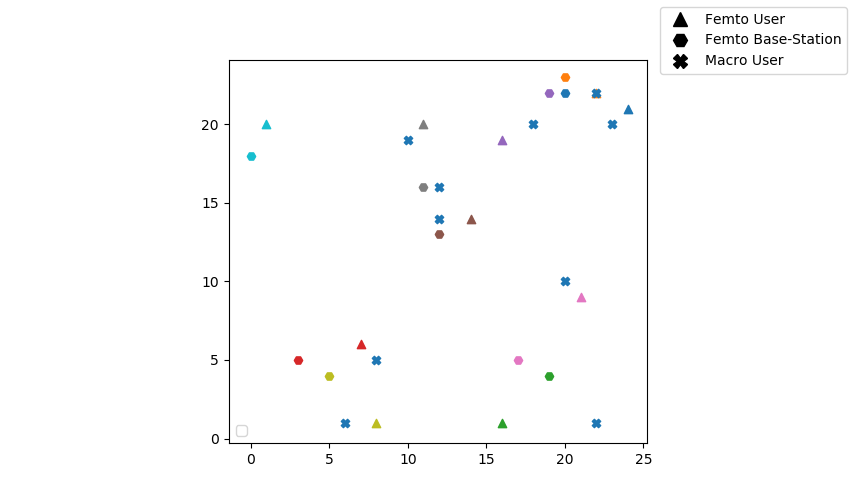
\includegraphics[width=\textwidth,height = 10cm]{figures/system_figure_single}
	  \caption{Simluation Setup Single Antenna and User.  }
\end{figure}

\begin{figure}[H]
	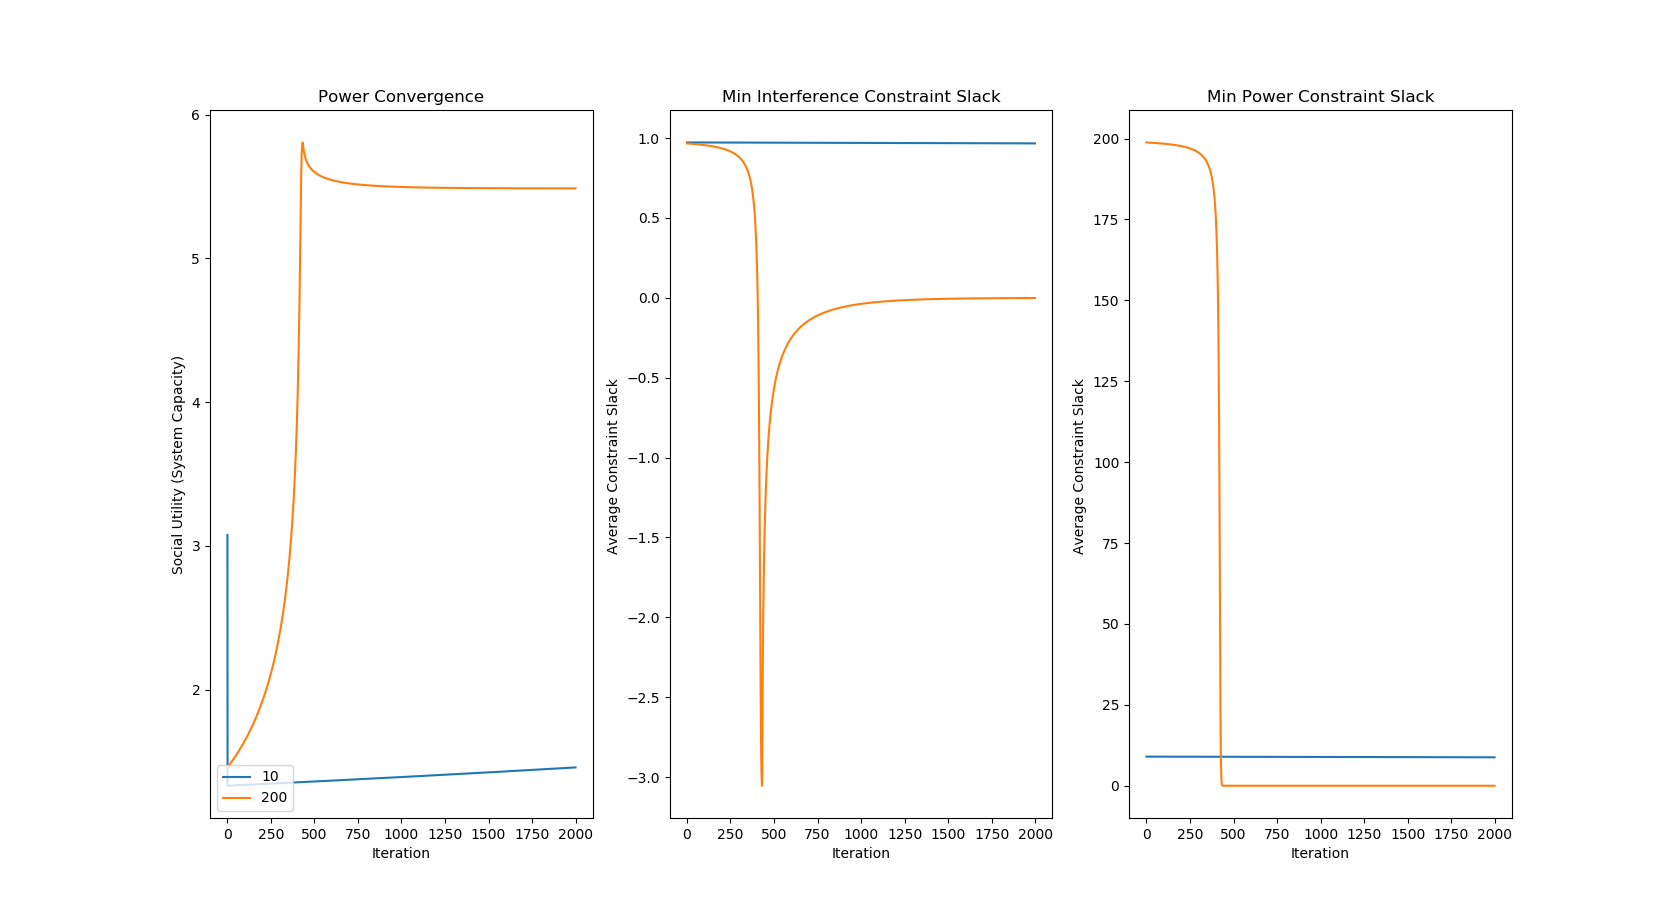
\includegraphics[width= 15cm,height = 10cm]{figures/single_power}
	  \caption{Single Antenna Game Simulation with different base station power constraints}
\end{figure}

\begin{figure}[H]
	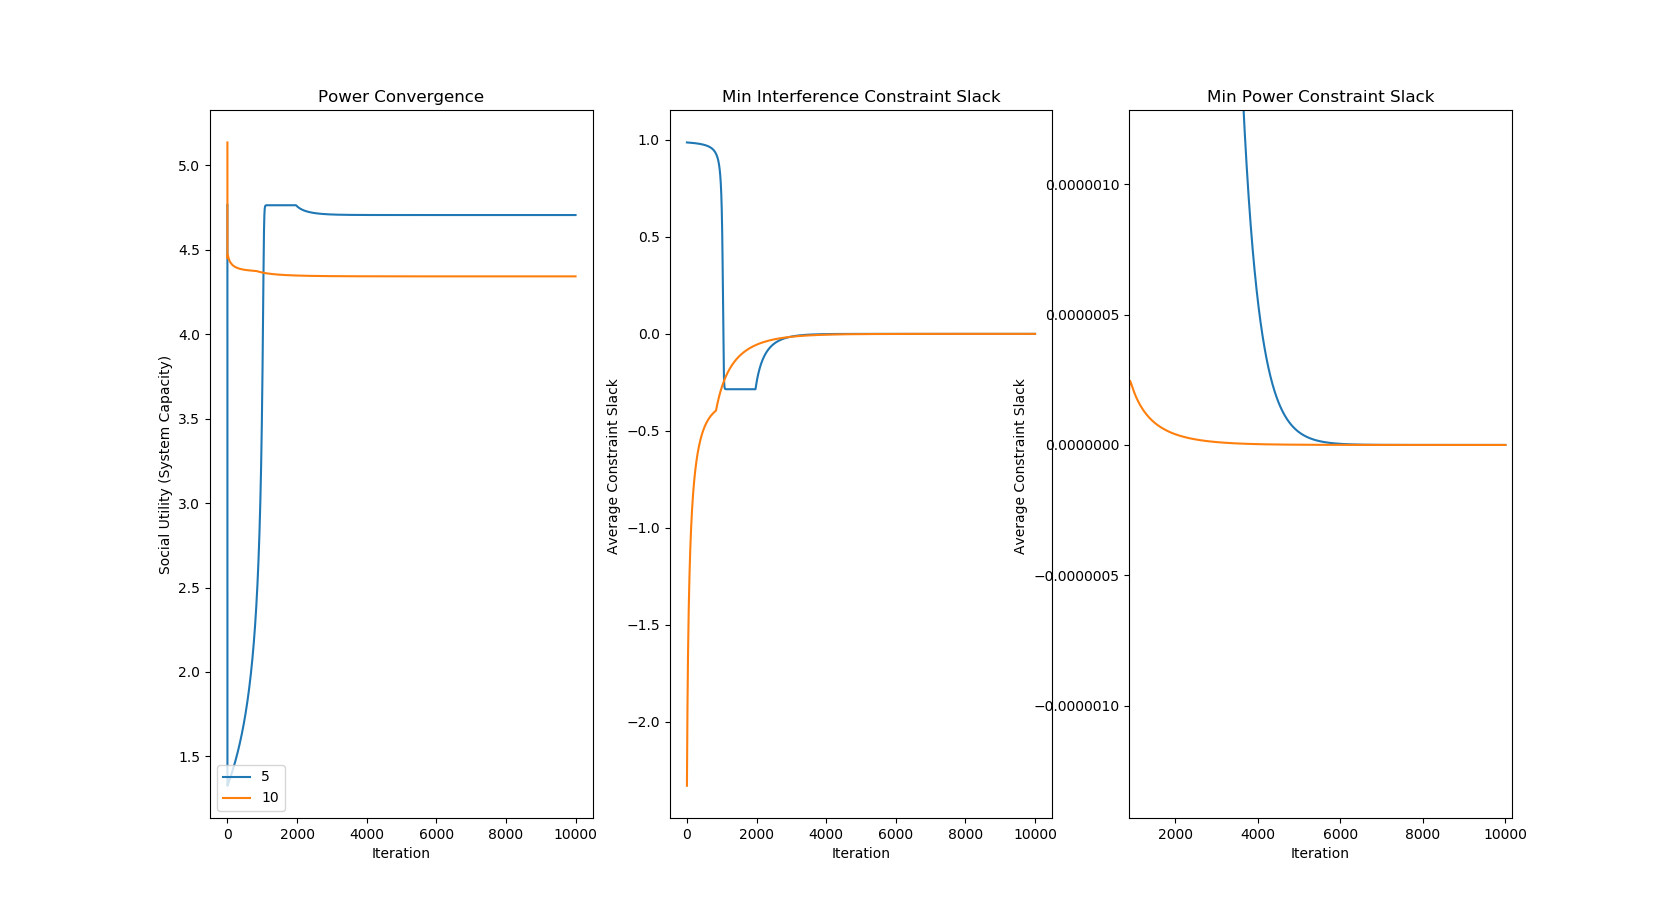
\includegraphics[width= 15cm,height = 10cm]{figures/single_macro}
	  \caption{Single Antenna Game Simulation with different numbers of macrocell users}
\end{figure}

\begin{figure}[H]
	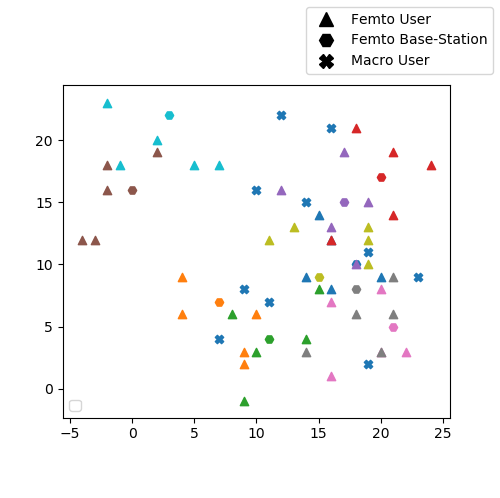
\includegraphics[width=\textwidth,height = 10cm]{figures/system_figure_multiple}
	  \caption{Simluation Setup Multiple Antenna and User.
	  }
\end{figure}


\begin{figure}[H]
	  	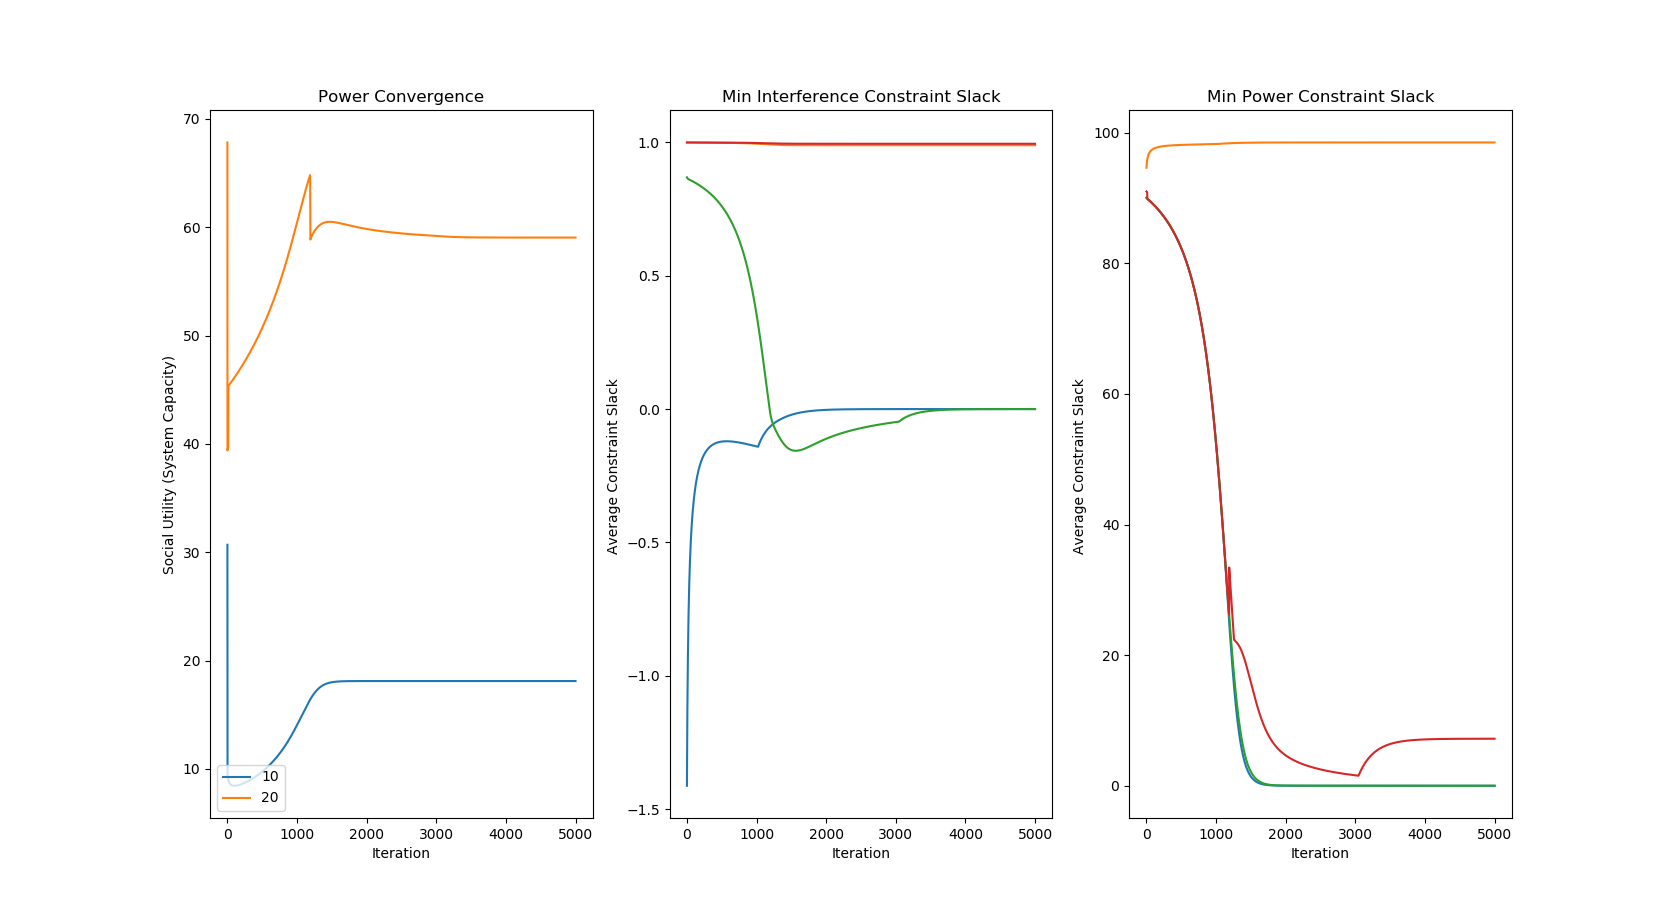
\includegraphics[width=\textwidth,height = 7cm]{figures/increasing_antenna}
	  		  \caption{Convergence for different numbers of antennas at FBSs. Number of femto cell users and macrocell users constant. Each BS has 10 users.}
	  \label{fig:}
\end{figure}

%
%\begin{figure}[H]
%	  	\includegraphics[width=\textwidth,height = 7cm]{figures/increasing_antenna_game_beam-former}
%	  		  \caption{Different choices for the zero-forcing beam-former $\mathbf{U}_{\text{f}}$}
%	  \label{fig:inc_fc}
%\end{figure}

%The concave setup of the FBS utility function is contingent upon knowledge of the channel state information $\mathbf{H}_{\text{f}}$. We now evaluate the effect of imperfect estimate of $\mathbf{H}_{\text{f}}$ on the solution. Imperfect CSi is simulated by adding additive white gaussian noise to the entries in $\mathbf{H}_{\text{f}}$. Need to check if this is even reasonable to simulate because might no longer be a game. TODO: Add Figure

%\begin{figure}[H]
%	  	\includegraphics[width=\textwidth,height = 7cm]{figures/increasing_antenna_game_beam-former}
%	  		  \caption{Impact of imperfect estimate of $\mathbf{H}_{\text{f}}$ at FBS $f$}
%	  \label{fig:inc_fc}
%\end{figure}


\chapter{Conclusion}
In this work, the power allocation problem for heterogeneous networks with MIMO capable basestations has been analyzed. The most general setup of this problem poses difficulties for distributed solutions due to the non-concavity of the resulting utility functions. It is shown that under additional beam-forming constraints on the MIMO capable base stations, a unique Nash Equilibrium can be achieved with a distributed solution. 
\par
Future work should extend the system presented here to further generalizations including interference between the femtocell basestations, and the potential for imperfect channel estimation. 
\newpage
\bibliography{gt_report}
\end{document}
